\documentclass[final, 3p, 11pt]{elsarticle}

% Packages
\usepackage{lmodern}
\usepackage[T1]{fontenc}
\usepackage{amsmath}
\usepackage{graphicx}
\usepackage{hyperref}
\usepackage{booktabs}
\usepackage{multicol}
\usepackage{subcaption}
\usepackage{listings} % For code

\usepackage[numbers]{natbib}
\bibliographystyle{plainnat}

\setlength{\parskip}{1em}
\setlength{\parindent}{0pt}

% Python code style settings
\lstset{language=Python, % Setting Python as the language
        basicstyle=\ttfamily\small, % Basic font style
        keywordstyle=\color{blue}, % Keywords in blue
        commentstyle=\color{green!50!black}, % Comments in green
        stringstyle=\color{red}, % Strings in red
        showstringspaces=false, % Don't show spaces in strings
        breaklines=true} % Line breaking

% Begin document
\begin{document}
\begin{frontmatter}

% Title Page

\title{Non-intrusive Testing of Liquid Culture Medium using Online NIR Spectroscopy and Machine Learning for Qualitative Analysis}

\author[1]{Benjamin Samuel\fnref{cor3}}
\author[1]{Connor Reintjes\fnref{cor1,cor2}}
\author[1]{Paola Gonz\'alez P\'erez\fnref{cor2}}
\author[1]{Shiza Hassan\fnref{cor3}}
\author[1]{\\Dr. Amin Reza Rajabzadeh\fnref{cor4}} % Supervisor as corref

\fntext[cor1]{Conceptualization} % Custom footnote for dry-lab-1
\fntext[cor2]{Validation \& Software} % Custom footnote for dry-lab-2
\fntext[cor3]{Investigation \& Methodology} % Custom footnote for wet-lab
\fntext[cor4]{Principle Investigator \& Capstone Supervisor} % Custom text for Supervisor

\affiliation[1]{organization={McMaster University, W. Booth School of Engineering Practice and Technology}, city={Hamilton, ON.}, country={Canada}}

\begin{abstract}
Insufficient quality assurance is a major expense associated with laboractories that an result in contamination, poor sample integrity, and lead to lost time due to repetitive sample testing. To ameliorate these issues, NIR spectroscopy has been combined with machine learning in this approach to qualitatively analyze the composition of liquid cultures in a non-intrusive and online manner. This will allow laboratories to save time by identifying contamination as soon as it happens and proceeding accordingly, as opposed to finding out after a full protocol has been performed. The method to achieve this involved creating a handheld casing to house the NIR which would take spectra of the sample and pass it to a machine learning model that would then identify whether the sample is in a normal or contaminated state. In phase 1 of the experiment, the NIR housing was built and initial testing was conducted for both contaminated and non-contaminated states, with the contaminant being Lactobacillus rhamnosus. The results achieved indicate that the NIR was able to differentiate between contaminated and non-contaminated samples. To analyze these readings a 1D-CNN model will be trained with the data collected thus far in the second phase of the experiment. Moving forward, further testing will be performed using quartz cuvettes to achieve more accurate and precise results as well as plating of bacteria to generate a standard curve to achieve quantitative results. 

\end{abstract}

\begin{keyword}
Bioprocess Monitoring \sep Machine Learning \sep Near-Infared Spectroscopy (NIR) \sep 1D Convolutional Neural Network (1D-CNN) \sep Qualitative Analysis
\end{keyword}

\end{frontmatter}

% Introduction
\section{Introduction}
Quality assurance issues are responsible for repeated testing, misdiagnosis, improper treatment and unpredictable costs \citep{randox_quality}. The contamination of samples is the most common problem experienced in microbial laboratories. The real-time monitoring of samples can represent a significant cost-saving solution to improve quality assurance practices in laboratory and industrial settings \citep{abatenh2018contamination}. To improve these issues, Near Infrared (NIR) spectroscopy has been combined with deep learning to provide real-time analysis of sample quality. This online analysis increases the testing and result obtention speed while remaining non-invasive to reduce further contamination of the samples \citep{sohn2021gmo}. This technology also symbolizes a financial advantage by reducing the loss of biological samples using low computational requirements that can measure and classify the analyzed data as required. A deep learning model will be used to optimize this analysis as it offers advantages such as automatically integrating feature extraction, and incorporating hundreds of layers with many parameters compared to artificial neural networks \citep{mishra2022hypes}.
The NIR spectral region has a range from 700 nm to 2500 nm. It is primarily characterized by absorption bands corresponding to the overtone and combination bands of C-H, N-H, O-H, and S-H stretching Figure \ref{fig:analytical_bands}. Hence, the spectra of most compounds will show unique absorption peaks in the NIR spectral region. These peaks can be used for the quantitative and qualitative analysis of the compounds in gases, solids or liquids.

        \begin{figure}[h]
                \centering
                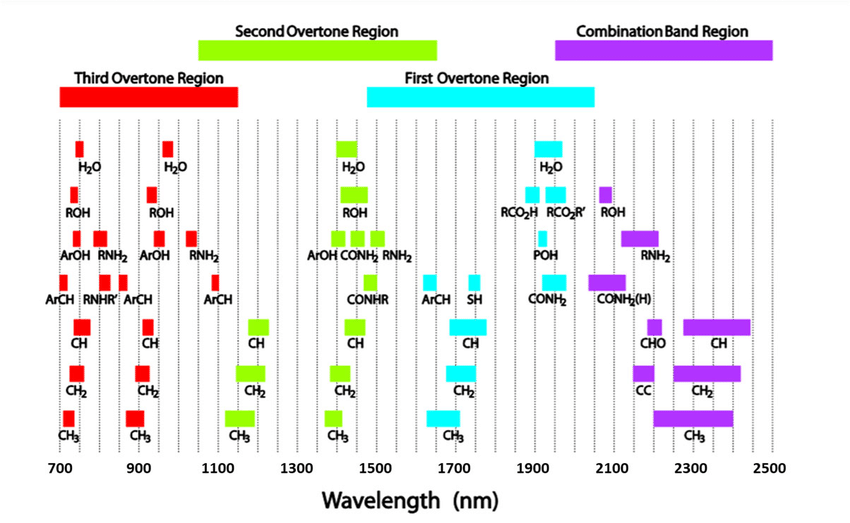
\includegraphics[width=0.5\textwidth]{Images/principle_analytical_bands.png}
                \caption{Principal analytical bands and relative peak locations for absorptions in the near-infrared region. Unique absorptions found in the majority of chemical and biological products can be utilized in both qualitative and quantitative examinations}
                \label{fig:analytical_bands}
                \end{figure}

Ethanol and water have characteristic NIR spectrum patterns that allow for their identification and quantification. Ethanol has a unique narrow peak at 1200 nm representing the second overtone of the C-H stretching vibration \citep{antonpaar_nir}. Water, on the other hand, shows a flat behaviour at this wavelength due to the lack of C-H bonds.

        \begin{figure}[h]
                \centering
                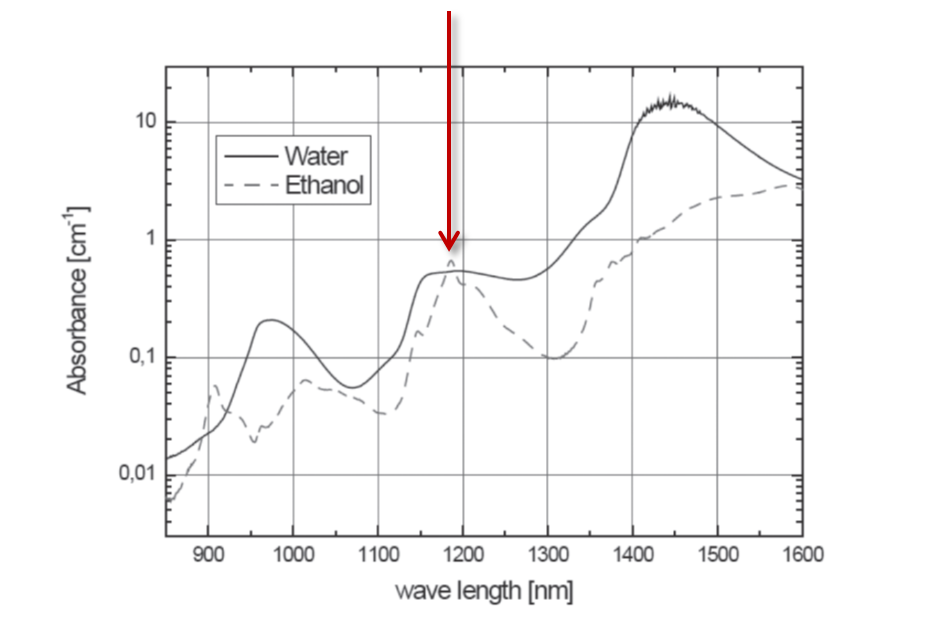
\includegraphics[width=0.5\textwidth]{Images/anton_paar.png}
                \caption{NIR spectrum of ethanol and water \citep{antonpaar_nir}}
                \label{fig:ethanol-water_curve}
                \end{figure}

The intensity of NIR absorption bands is 10–100 times lower than that of the equivalent basic mid-IR absorption bands. This facilitates the direct analysis of strong absorbances and high light-scattering efficiency. Band overlap and penetration depth reduce in the near-infrared (NIR) spectral region, whereas the efficiency of light scattering and absorptivity improves with wavelength. As NIR spectroscopy depends on light absorption, spectral data can be acquired either in transmittance or reflectance mode. Diffuse reflectance $(\log(\frac{1}{R}))$ measurements are favored for opaque or light-scattering matrices whereas translucent samples used transmittance $(\log(\frac{1}{R}))$.
NIR spectroscopy's quickness, adaptability to a variety of materials, and capacity to examine liquid samples make it a promising tool for bio applications \citep{becInfraredSpectroscopyBioApplications2020}. Recent advancements are making NIR spectroscopy more accessible with portable handheld instruments that allow for real-time, on-site examination. 

Cell culture media (CCM) plays a vital role, directly impacting process yield and product quality \citep{ryderCellCultureMedia2018}. CCM's primary objective is to create and sustain an optimal physiological environment for large-scale cell culturing, ensuring cell health and expression of desired Critical Quality Attributes (CQAs). However, it's crucial to recognize that the chemical and physical properties of CCM are sensitive to microbial growth, chemical reactions, and environmental factors like temperature and light. Without sterilization, CCM can rapidly change due to microbial contamination, leading to increased turbidity and light scatter, consequently elevating baselines and noise in spectra, potentially compromising measurements. While chemometrics can mitigate some measurement errors, identifying errors induced by samples and measurements in CCM analysis can be challenging.

NIR spectra are known to be high-dimensional data due to the baseline drift and other noise signals present. This results in the need for preprocessing techniques for noise filtering and dimensionality reduction before analyzing the true compound signals. Hence, NIR spectra usually involve the use of chemometric algorithms like partial least squares regression (PLSR) and support vector regression (SVR) to clean the data from baseline drift as well as to understand the chemical changes in the samples \citep{shangNIRSpectroscopyCombined2023,naguib2014support}. These algorithms require trained individuals to obtain the necessary parameters used to analyze the spectra \citep{wang2021fcnn}. Similarly, chemometric models are often limited by their inability to generalize for variance in spectra from different instruments, or changing storage and growing conditions (P03). Deep Learning Machine Learning (ML) can be used to automate extracting the main compound features from high-dimensional spectral data and eliminate the need for feature-selection techniques \citep{walsh2023fruit}. 

While different classes of ML algorithms have successfully achieved the classification of NIR spectra, traditional ML methods such as partial least squares (PLS), K-nearest neighbor (KNN), and principal component analysis (PCA) require a higher level of expertise to design suitable features of the model’s architecture \citep{zhangReviewMachineLearning2022}. Deep learning, on the other hand, does not require a high level of expertise as it utilizes the raw features of data to analyze and classify it as needed. This is achieved through multiple hidden layers that are trained end to end. Some of these layers can be specialized convolution layers that allow for the learning and identification of local feature patterns. This aspect enables deep learning architectures to employ less preprocessing for high-dimensional data \citep{yue2021intrusion}. 

Convolutional neural networks (CNNs) are a class of deep neural networks commonly used for data analysis due to their successful results in image processing and classification \citep{sharma2018cnn}, speech recognition, and other computer vision tasks. CNNs are a feed-forward multi-layer architecture in which a kernel or filter takes specific features from local regions from the upper layer. This architecture allows for an autonomous extraction of important features from complex data for analysis and learning \citep{zhangReviewMachineLearning2022}. A common drawback of the use of CNNs for spectral analysis is the requirement of large data sets during the training process of the model. To avoid overfitting due to a limited number of data samples, one-dimensional CNN (1D-CNN) can be used. These models are similar to traditional CNNs except for the data size required and low computational requirements. 1D-CNNs have proven to have good information extraction and high classification accuracy with simple preprocessing techniques. It has been applied by \citep{shangNIRSpectroscopyCombined2023} for the analysis and classification of NIR spectra from breast cancer tissue to aid in cancer diagnosis, demonstrating a $94.67\%$ classification accuracy. \citet{chaiImproved1DConvolutional2021} also developed an improved 1D-CNN structure to discriminate Anoectochilus roxburghii from its counterfeits using NIR spectra.

Previous studies performed on 1D-CNN for the analysis of NIR spectral data demonstrate the viability of its application for the online analysis of culture media. The present study aims to develop a method based on NIR spectra acquired on a portable device, as a non-destructive, online method to assess quality attributes of culture media. Due to the expected nature of the data collection, it was necessary to employ a time series analysis when designing the CNN structure. Within this experiment S. cerevisiae was used as the model, testing it under two conditions, normal and contaminated with Lactic Acid Bacteria. Lactobacillus rhamnosus was used as the contaminant of choice due to its improved growth in the presence of S. cerevisiae. Also, using this species ensures the proper growth of S. cerevisiae as it remains unaffected in its presence \citep{nenciarini2023yeast}. The NIR spectra of ethanol were analyzed in each case and passed to the deep learning model which classified the “normal” baseline against a “non-normal” sample. 

\section{Materials and Methods}
\subsection{Materials}
\subsubsection{Material List}
\begin{table}[ht]
        \centering
        \begin{tabular}{l l l l l l}
        \toprule
        Item & Supplier & Catalog Number & Quantity & Price & URL \\
        \midrule
        S. Cerevisiae & Sigma Aldrich & YSC1 & 100g & \$192 CAD & \href{https://www.sigmaaldrich.com/CA/en/product/sigma/ysc1}{Link} \\
        Peptone & Sigma Aldrich & 68727 & 5g & \$165 CAD & \href{https://www.sigmaaldrich.com/CA/en/product/sial/68727?icid=sharepdp-clipboard-copy-productdetailpage}{Link} \\
        Yeast Extract & Sigma Aldrich & Y6125 & 5g & \$119 CAD & \href{https://www.sigmaaldrich.com/CA/en/product/sigma/y1625?icid=sharepdp-clipboard-copy-productdetailpage}{Link} \\
        Dextrose & Sigma Aldrich & G7021 & 10g & \$74 CAD & \href{https://www.sigmaaldrich.com/CA/en/search/dextrose?focus=products&page=1&perpage=30&sort=relevance&term=dextrose&type=product}{Link} \\
        CytoSoft®T-25 Flasks & Sigma Aldrich & CC330 & 1x * 10 & \$247 CAD & \href{https://www.sigmaaldrich.com/CA/en/product/mm/cc330}{Link} \\
        ABS Filament & Bambu Lab & ABS Black w/ Spool & 1x 1kg & \$35.99 CAD & \href{https://ca.store.bambulab.com/products/abs-filament?variant=44183939580144}{Link} \\
        Lacticaseibacillus rhamnosus & ATCC & 7469 & 1 vial & - & \href{https://www.atcc.org/products/7469}{Link} \\
        \bottomrule
        \end{tabular}
        \caption{Material Information Table with URLs}
        \label{tab:matinfo}
        \end{table}

\subsubsection{NIR Housing Design}
Due to the design of the DLP NIRscan Nano (Texas Instruments) and the location of the sensor window on the unit, it required a housing to be designed. This housing was designed to both hold the NIR as well as the sample to ensure consistent scan conditions. The housing was created using a 3D printer (P1S, Bambu Labs) using Matte PLA filament (Bambu Labs) for the test models, and was reprinted in ABS filament (Bambu Labs) for the final housing. 
The housing underwent multiple iterations with all design and modeling performed within AutoDesk Fusion360 parametric CAD software. The final iteration of the housing used can be seen below in Figure 2. All of the components slide along a single dovetail mount along the bottom plate to allow for quick assembly while keeping all components secure. Due to slight problems with temperature regulation, a NF-A4x10 5V PWM fan from Noctua was added in addition to a fan speed controller (NA-FC1), to prevent the NIR from overheating during scans. A cuvette holder was also designed to allow for the quick change of samples, while also ensuring that the cuvette remained fixed in place for scans. 

\begin{figure}[ht]
        \centering
        \begin{subfigure}[b]{0.45\textwidth}
            \centering
            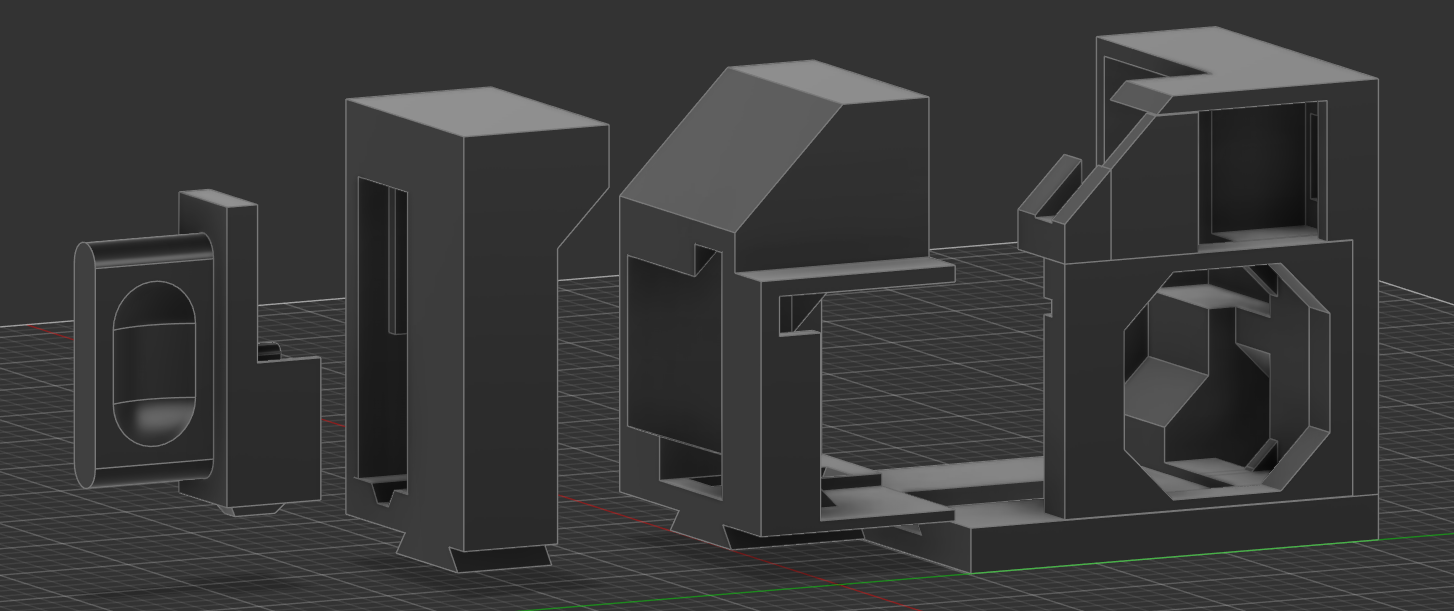
\includegraphics[width=\textwidth]{Images/nir_exploded.png}  % Replace with your image file
            \caption{NIR Housing Exploxed}
            \label{fig:subfigure1}
        \end{subfigure}
        \hfill
        \begin{subfigure}[b]{0.45\textwidth}
            \centering
            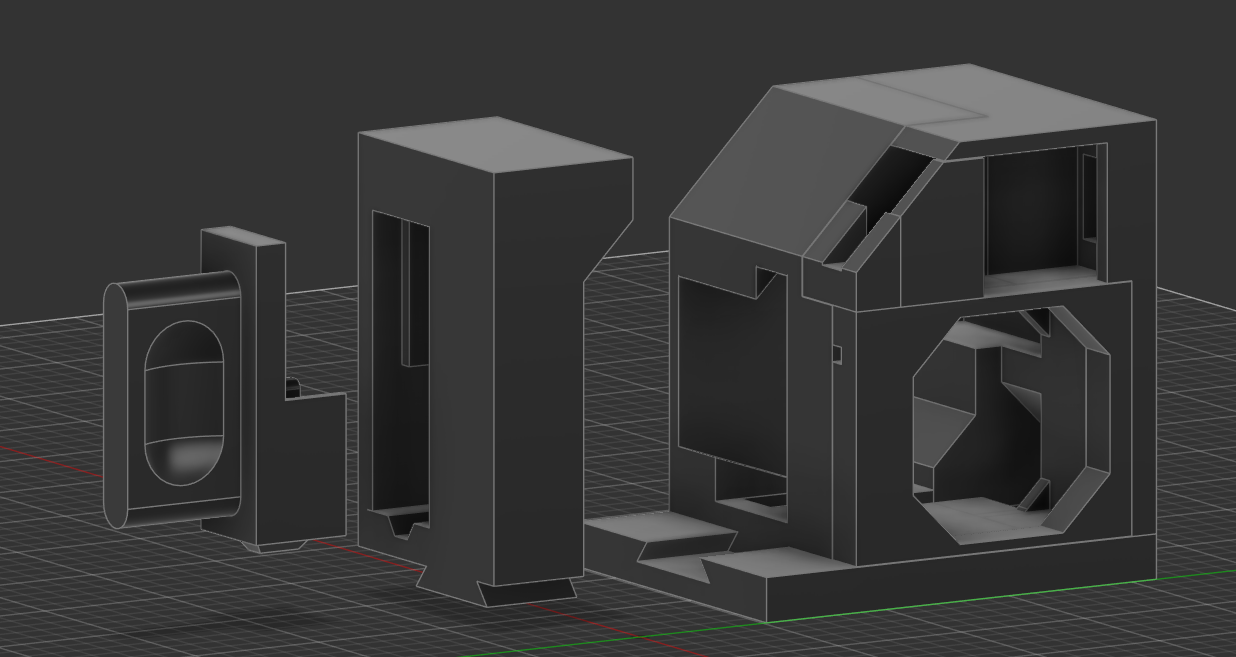
\includegraphics[width=\textwidth]{Images/nir_housing.png}  % Replace with your image file
            \caption{NIR Housing Un-Exploded}
            \label{fig:subfigure2}
        \end{subfigure}
        \caption{Combined Images as Subfigures}
        \label{fig:combinedfigures}
    \end{figure}


\subsection{Methods}
Methods

\section{Results}
Results

\subsection{Data Analysis}
Analysis

\section{Discussion}
Discussion

\section{Conclusion}
Conclusion

\section*{Acknowledgments}
Acknowledge any individuals or organizations that contributed to the research, funding bodies, and any supporting institutions.

\newpage
\bibliography{references}     % The .bib file name (without the .bib extension)

% End document
\end{document}
